\documentclass[12pt, a4paper]{article}

\usepackage[utf8]{inputenc}
\usepackage[spanish]{babel}
\usepackage{titling}
\usepackage[left=2cm,right=2cm,top=2cm,bottom=2cm]{geometry}
\usepackage{enumerate}
\usepackage{amsmath}
\usepackage{graphicx}

\usepackage{listings}%-para agregar codigo-
\usepackage[usenames,dvipsnames]{color}
\usepackage{color}%------------------------

%---------------------importar codigo desde archivos cpp----------------------------
\lstloadlanguages{C++}
\lstnewenvironment{code}
	{%\lstset{	numbers=none, frame=lines, basicstyle=\small\ttfamily, }%
	 \csname lst@SetFirstLabel\endcsname}
	{\csname lst@SaveFirstLabel\endcsname}
\lstset{% general command to set parameter(s)
	language=C++, basicstyle=\small\ttfamily, keywordstyle=\slshape,
	emph=[1]{tipo,usa}, emphstyle={[1]\sffamily\bfseries},
	morekeywords={tint,forn,forsn},
	basewidth={0.47em,0.40em},
	columns=fixed, fontadjust, resetmargins, xrightmargin=5pt, xleftmargin=15pt,
	flexiblecolumns=false, tabsize=2, breaklines,	breakatwhitespace=false, extendedchars=true,
	numbers=left, numberstyle=\tiny, stepnumber=1, numbersep=9pt,
	frame=l, framesep=3pt,
    basicstyle=\ttfamily,
    keywordstyle=\color{blue}\ttfamily,
    stringstyle=\color{magenta}\ttfamily,
    commentstyle=\color{RedOrange}\ttfamily,
    morecomment=[l][\color{OliveGreen}]{\#}
}

\lstdefinestyle{C++}{
	language=C++, basicstyle=\small\ttfamily, keywordstyle=\slshape,
	emph=[1]{tipo,usa,tipo2}, emphstyle={[1]\sffamily\bfseries},
	morekeywords={tint,forn,forsn},
	basewidth={0.47em,0.40em},
	columns=fixed, fontadjust, resetmargins, xrightmargin=5pt, xleftmargin=15pt,
	flexiblecolumns=false, tabsize=2, breaklines,	breakatwhitespace=false, extendedchars=true,
	numbers=left, numberstyle=\tiny, stepnumber=1, numbersep=9pt,
	frame=l, framesep=3pt,
    basicstyle=\ttfamily,
    keywordstyle=\color{blue}\ttfamily,
    stringstyle=\color{magenta}\ttfamily,
    commentstyle=\color{RedOrange}\ttfamily,
    morecomment=[l][\color{OliveGreen}]{\#}
}

\def\nbtitle#1{\begin{Large}\begin{center}\textbf{#1}\end{center}\end{Large}}
\def\nbsection#1{\section{#1}}
\def\nbsubsection#1{\subsection{#1}}
\def\nbcoment#1{\begin{small}\textbf{#1}\end{small}}
\newcommand{\comb}[2]{\left( \begin{array}{c} #1 \\ #2 \end{array}\right)}
\def\complexity#1{\texorpdfstring{$\mathcal{O}(#1)$}{O(#1)}}
 \newcommand\cppfile[2][]{
\lstinputlisting[style=C++,linerange={#1}]{#2}
}
%%------------------------------------------------------------------------------

\newcommand{\subtitulo}[1]{\begin{center}\textbf{#1}\end{center}}

\title{\textbf{Programación Dinámica}}
\author{Wilmer Emiro Castrillón Calderón}

\begin{document}
	\maketitle
	
	La programación dinámica es una metodología utilizada para reducir la compejidad computacional a un
	algoritmo, es usada principalmente para resolver problemas de optimización,
	se basa en la estrategia \textit{divide y venceras}, consiste en tomar un problema complejo y dividirlo 
	sucesivamente en sub-problemas mas pequeños hasta llegar a un caso base, y partir de ahí empezar a construir la
	solucion de cada sub-problema, hasta llegar a una solución global. Durante la busqueda de soluciones
	se utiliza tablas de memorización, en la cuales se iran guardando la solucion óptima de cada sub-problema.
	Como abrebiatrura a programnación dinámica vamos a usar dp, pues son sus siglas en ingles.
	
	Un problema se puede resolver usando programación dinámica si cumple con tres condiciones basicas:
	\begin{enumerate}[1.]
		\item El problema se puede dividir en sub-problemas, y estos a su vez en más sub-problemas, y así hasta llegar
				a un caso base.
		\item La solución óptima de cada sub-problema depende de la solución óptima de cada uno de sus
				propios sub-problemas, entonces cumple con el principio de optimalidad de Bellman.
		\item Se presenta superposición de problemas, osea que hay sub-problemas que aparecen multiples veces
		 		a lo largo de la busqueda de la solución general. Aunque como tal no es obligatorio, es la razón 
		 		principal que le permite tener menor complejidad computacional.
	\end{enumerate}
	
	\subtitulo{Ejemplo inicial.}
	
	El ejemplo basico más usado es con la sucesión de fibonacci, esta comienza con los números 0 y 1 y a partir
	de estos dos el siguiente número es la suma de los dos anteriores y así hasta infinito, los primeros
	numeros son los siguientes:
	\begin{center} $0, 1, 1, 2, 3, 5, 8, 13, 21, 34, 55, 89, ..... $ \end{center}
	
	Ahora vamos a buscar la manera de calcular y guardar los primeros n numeros de la serie eficientemente, 
	guardaremos en un vector los elementos de la sucesión, de tal forma que la posición i-esima del vector
	corresponda al número i-esimo de la serie.
	
	 Para solucionar el problema con dp primero debemos identificar
	los subproblemas, esto siempre resulta en una formula recursiva, en este caso es la siguiente:\\
	$f(n) = 	
		\begin{cases}
			n & \text{if $n\le 1$}\\
			f(n-1) + f(n-2) & \text{if $n\ge 2$}
	\end{cases}	$\\
	
	Para implementar dp surgen dos enfoques: Top-Down y Buttom-Up, vamos a resolver este ejemplo usando los dos.\\
	
	\textbf{Buttom-Up}\\
	En este enfoque vamos a ir recorriendo la tabla de memorización mientras la llenamos, comenzando desde los
	casos base de la formula recursiva y apartir de ahí ir calculando y guardando los demas resultados de la
	tabla. Para este ejercicio comenzamos llenando en un vector \textit{v} los casos
	base: \textit{v[0] = 0; v[1] = 1;} y luego llenamos el resto del vector según nos indica la formula
	recursiva: \textit{v[i] = v[i-1] + v[i-2]}, de tal forma que \textit{v[i-1]} y \textit{v[i-2]} son valores
	que hemos calculado antes y ademas $v[x] = f(x)$. A continuación se muestra un ejemplo en c++:
	\cppfile[5-12]{codigos/fibo.cpp}
	Aunque en este enfoque no utilizamos llamados recursivos, puede resultar mas dificil de implementar,
	pues por lo general es menos intuitivo.\\
	
	\textbf{Top-Down}\\
	A diferencia del anterior enfoque, en este vamos a utilizar llamados recursivos, los cuales mientras se
	realizan se iran guardando sus resultados en la tabla de memorización, y así evitar calcular dos veces el
	mismo llamado recursivo. En este enfoque se hace mas notorio la importacia de la tabla de memorización, 
	veamos la eficiencia del algoritmo si dejamos unicamente la formula recursiva, el codigo seria el siguiente:
	\cppfile[14-20]{codigos/fibo.cpp}
	Si ejecutamos este codigo para $fibo(6)$ obtenemos el siguiente arbol de recursión:\\
	\begin{center}
		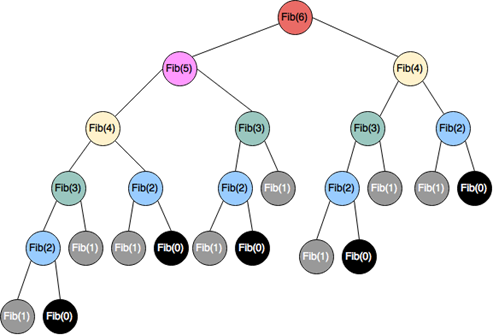
\includegraphics[scale=0.92]{imagenes/arbol_recursion}
	\end{center}
	
	Se puede observar que se realizan multiples llamados repetidos, $fibo(4)$ se repite 2 veces, $fibo(3)$
	3 veces, $fibo(2)$ 4 veces, $fibo(1)$ 8 veces y $fibo(0)$ 5 veces, resultan bastantes llamados recursivos
	solamente para encontrar $fibo(6)$, esta solución tiene ¡una complejidad exponencial!, en numeros pequeños
	no es muy notorio pero cuando intentamos encontrar $fibo(42)$ o $fibo(45)$ el tiempo de ejecución se hace
	muy alto, entonces para mejorar tiempos se debe implementar una tabla de memorización en la cual guardaremos
	el resultado de cada llamado recursivo y agregamos un condicional al inicio del metodo preguntando si la
	solución de ese sub-problema ya fue encontrada, en tal caso se devuelve el valor guardado sino se calcula y se
	guarda, la tabla comenzara llena con -1, de tal forma que si una casilla es -1 entonces se debe calcular.
	\cppfile[22-31]{codigos/fibo.cpp}
	Este ejercicio resulta muy trivial, se puede resolver facilmente sin pensar en dp, ahora se mostraran
	multiples problemas en los cuales se hace necesario utilizar dp para dar una solución eficiente.
	
	\subtitulo{Recorrido óptimo en una matriz.}
	
	Teniendo una matriz de n x m con números enteros, se quiere conocer la suma maxima que se puede obtener
	recorriendo la matriz, comenzando desde la esquina superior-izquierda y terminando en la esquina inferior-derecha
	únicamente haciendo pasos hacia la derecha y abajo, por ejemplo:\\
	\begin{center}
		\begin{tabular}{|l|l|l|}
			\hline
			5  &6 &4 \\ \hline
			3  &8  &5 \\ \hline
			2 &11 &15 \\ \hline
			5 &2  &17 \\ \hline
		\end{tabular}
	\end{center}
	El camino óptimo es 5-6-8-11-15-17 y la suma es 62.\\
	
	Este es un problema de optimización, a simple vista una posible solución seria siempre ir a la casilla adyacente
	con mayor valor, pero no siempre es la mejor, por ejemplo teniendo la siguiente matriz:
	\begin{center}
		\begin{tabular}{|l|l|l|l|}
		 	\hline
			1  & 12 & 4  & 9 \\ \hline
			6  & 5  & 21 & 15 \\ \hline
			35 & 18 & 8  & 10 \\ \hline
			12 & 2  & 4  & 15 \\ \hline
		\end{tabular}
	\end{center}
	No es una solución óptima ir a la siguiente casilla con mayor valor, pues haciendo esto se tendria el siguiente
	camino 1-12-5-21-15-10-15 con un acumulado de 79, en cambio el camino 1-6-35-18-8-10-15 tiene un acumulado de 93,
	necesitamos encontrar la suma del camino óptimo.\\
	
	Este problema se puede resolver con programación dinámica, pues podemos encontrar la solución general a
	partir de la solución de sub-problemas más pequeños, supongamos	que tenemos una matriz T de tamaño n x m
	a la cual vamos a calcular la suma de su recorrido óptimo, para facilidad vamos a indexar desde 1 tomando
	la esquina superior-izquierda como T[1][1], para encontrar el camino óptimo hasta T[n][m](ultima casilla)
	es necesario primero encontrar el óptimo de T[n-1][m] y T[n][m-1], pues para llegar a T[n][m] hay dos opciones,
	llegar por arriba (equivalente a tomar la desición ir-abajo desde T[n-1][m]) o llegar por la izquierda 
	(equivalente a tomar la desición ir-derecha desde T[n][m-1]), entonces la solucion general sera 
	\textit{T[n][m] + maximo entre(camino óptimo hasta T[n-1][m], camino óptimo hasta T[n][m-1])}, y a su vez
	el óptimo para ellos se calcula de manera similar, el optimo para llegar hasta T[n-1][m] es 
	\textit{T[n-1][m] + maximo entre(camino óptimo hasta T[n-2][m], camino óptimo hasta T[n-1][m-1]).} y 
	así tambien para T[n][m-1], de esta forma podemos dividir el problema en sub-problemas.\\
	
	Ahora ya podemos ir construyendo una formula recursiva, pero nos faltan los casos base, entonces llamaremos
	$i$ a la posicion en fila y $j$ a la posición en columna, ahora si $i$ y $j$ son iguales a 1 entonces
	el resultado es T[1][1], si solo $i$ es 1 entonces el resultado es \textit{T[1][j] + camino óptimo hasta T[1][j-1]},
	solo podemos llegar desde la izquierda pues por arriba nos estariamos saliendo de la matriz, si solo $j$
	es 1 entonces de manera similar tenemos \textit{T[i][1] + camino óptimo hasta T[i-1][j]}, ahora ya tenemos
	los casos base y podemos construir la formula recursiva:\\
	$f(i, j) = 	
		\begin{cases}
			T[1][1] & \text{if $i,j = 1$}\\
			T[1][j] + f(1, j-1) & \text{if $i = 1$}\\
			T[i][1] + f(i-1, 1) & \text{if $j = 1$}\\
			T[i][j] + mayor(f(i-1, j), f(i, j-1)) & \text{if $i,j \neq 1$}
		\end{cases}
	$\\
	Como tabla de memorización vamos a tomar otra matriz de igual tamaño, a esta la llamaremos memo, en ella iremos
	guardando el acumulado óptimo, o sea que en memo[i][j] se guardara el acumulado óptimo para ir desde
	T[1][1] hasta T[i][j], ahora podemos solucionar el problema usando cualquiera de los dos enfoques de dp,
	para usar Top-Down solamente le agregamos la tabla de memorización a la formula recursiva y se tendria
	solucionado el problema.
	\cppfile[8-19]{codigos/matriz.cpp}
	
	para conocer el resultado solo imprimimos $f(n-1, m-1)$  pues en c++ indexamos desde cero. Una solución con
	Buttom-Up es recorrer la matriz y llenarala segun la formula recursiva, se debe comenzar llenando los casos
	base antes de calcular lo demas, para conocer la respuesta solo se llama el metodo y se imprime 
	$memo[n-1][m-1]$.
	\cppfile[22-35]{codigos/matriz.cpp}
	y ya tenemos solucionado el problema.\\
	
	\subtitulo{Suma de subconjuntos:}
	
	Tambien conocido como \textit{Sub-SetSum} el problema consiste en que teniendo un conjunto de números enteros
	$V$, encontrar si es posible que uno o multiples números $n$ sean el resultado de la suma de los elementos
	de un subconjunto del conjunto $V$, por ejemplo con el conjunto {1, 2, 5} es posible formar los numeros
	{1, 2, 3, 5, 6, 7, 8}.\\
	
	Con dp buscaremos todas las posibles sumas que se pueden formar con los números de un vector $v$ de tamaño $n$,
	por facilidad para este ejemplo vamos a indexar desde 1, para dar solución primero vamos a identificar los
	sub-problemas, la solución general incluye sumar el elemento $v[n]$ a todos los números encontrados
	hasta $v[n-1]$, y este a su vez depende de encontrar $v[n-2]$ y así sucesivamente hasta llegar a $v[1]$
	que sera nuestro caso base, mas detalladamente la solución hasta $v[1]$ es solamente él mismo, las soluciones
	hasta $v[2]$ es él mismo, $v[1]$ y la suma $v[1]+v[2]$, el cojunto de soluciones hasta ahora es
	\{$v[1]$, $v[2]$, $v[1]+v[2]$\}, ahora la solución hasta $v[3]$ sera
	\{$v[1]$, $v[2]$, $v[1]+v[2]$, $v[1]+v[3]$, $v[2]+v[3]$, $v[1]+v[2]+v[3]$\}, y así sucesivamente hasta $v[n]$,
	en este conjunto los numeros repetidos seran descartados.\\
	
	Por ejemplo supongamos que tenemos \{3, 5 y 8\}, la solución hasta 3 es él mismo, nuestro conjunto de soluciones hasta
	ahora es \{3\}, las soluciones hasta 5 es él mismo y su suma a las soluciones anteriores, nuestro conjunto de
	soluciones ahora es \{3, 5, 8\} y por ultimo incluyendo el 8, nuestro conjunto de soluciones queda de la siguiente
	forma: \{3, 5, 8, 11, 13, 16\}.\\
	
	Esto se puede resolver recursivamente con Top-Down pero quedara como tarea para el lector, áca se usara una solución
	iterativa usando Buttom-Up, para tabla de memorización usaremos una matriz con una cantidad de filas igual o mayor
	a la longitud del vector y de columnas igual al resultado más grande que se puede obtener, sera de tipo \textit{bool}
	pues el problema solo requiere decir si un numero se puede formar o no, cada fila i representara las soluciones
	encontradas hasta el $v[i]$.
	\cppfile[8-24]{codigos/SubSetSum.cpp}
	En el anterior codigo tomamos el vector $num$ como el conjunto de números $v$, tenemos dos ciclos el primero
	recorrera el vector $num$ y el segundo buscara las soluciones anteriores y le sumara a esa solución $num[i]$,
	como el caso base es cuando $i=0$ entonces debemos saltarnos el segundo ciclo, pues resulta innecesario
	porque no hay soluciones anteriores, para eso ponemos un condicional que ejecute el segundo ciclo si
	$i$ es mayor a 0, y por último si queremos saber si un número $m$ se puede formar entonces cosultamos en
	la última fila de la tabla de memorización, si $memo[num.size()-1][m]$ es verdadero entonce si existe un 
	sub-conjunto que sume $m$,
	en caso contrario no es posible formar esa suma.

	
	\subtitulo{Otros problemas clásicos:}
	
	\textbf{Problema de la mochila:} teniendo una mochila de capacidad $n$, un conjunto de objetos con peso $m$ 
	y una ganancia $c$, se debe encontrar la máxima ganancia que se puede guardar en la mochila sin
	exceder su capacidad.\\
	
	\textbf{Max Range Sum:} Dado un arreglo X de números enteros positivos y negativos, se debe encontrar la
	máxima suma que se puede lograr sumando posiciones consecutivas del arreglo.\\
	
	\textbf{Dominos en un tablero de 2*N:} consiste en encontrar la cantidad total de maneras en las que se puede
	llenar un tablero de tamaño 2*N con fichas de domino de tamaño 2X1, el tablero se debe llenar completamente sin
	tener espacios vacíos.
	
	\subtitulo{Bibliografia}
http://trainingcamp.org.ar/anteriores/2017/clases.shtml.\\
http://programacioncompetitivaufps.github.io/\\
https://www.geeksforgeeks.org/dynamic-programming-subset-sum-problem/\\
libro: competitive programming 3.\\



\end{document}



